\documentclass[usenames,dvipsnames]{beamer} %aby slo tvorit barvy

%%%%%%%%%%%%%%%%%%%%%%%%%%%%%%%%%%%%%%%%%%%%%%%
%makra vlozeni
%%%%%%%%%%%%%%%%%%%%%%%%%%%%%%%%%%%%%%%%%%%%%%%
\usepackage{amsmath}
\usepackage{tikz}
\usepackage{mathdots}
\usepackage{yhmath}
\usepackage{cancel}
\usepackage{color}
\usepackage{xcolor} %zakladnich 68 barev
\usepackage{siunitx}
\usepackage{array}
\usepackage{multirow}
\usepackage{amssymb}
\usepackage{gensymb}
\usepackage{tabularx}
\usepackage{booktabs}
\usetikzlibrary{fadings}
\usetikzlibrary{patterns}
\usetikzlibrary{shadows.blur}
\usepackage{setspace}
\usepackage{wrapfig}
\usepackage{pict2e}
%wraping text around table or picture

%  Kódování výstupu - aby šlo z pdf kopírovat včetně háčků a čárek

\usepackage[T1]{fontenc}
%  Základní typografická pravidla češtiny/slovenštiny

\usepackage{hhline}
%  moznost delat dvojite podtrezeni v tabulce 


%  Umožňuje použít dva obrázky vedle sebe
\usepackage{subcaption}

\linespread{1.1}
%  Po desetinné čárce v matematickém módu se nevytvoří mezera

\usepackage{icomma}
%  Pro vkládání obrázků ve formátu eps (např. z gnuplot)

\usepackage{epstopdf}

%  Automaticky odsadí i první paragraf v každé sekci
\usepackage{indentfirst}

%  Umožňuje rozdělovat obsah na více sloupců
\usepackage{multicol}
\usepackage{multirow}
\usepackage{booktabs}
%\usepackage{pgffor}


%  Lepší zobrazování matematiky (rozšíření sum o \limits atd.)
\everymath{\displaystyle}

%  Široké spektrum příkazů pro matematiku
% (Umožní např. psát přes \mathbb{N/R/Q/..} množiny čísel)
\usepackage{amsmath,amssymb}
\usepackage{amsfonts}
%  Velikost fontu matematických výrazů v dokumentu lze pro danou
% základního fontu dokumentu upravit pomocí:
% \DeclareMathSizes{X}{Y}{Z}{U} kde:
% X je velikost fontu v dokumentu, pro kterou se matematika upraví
% Y je standartní velikost fontu matematiky
% Z je velikost fontu zmenšených (vnořených výrazů)
% U je velikost fontu ještě více zmenšených (vnořených výrazů).
%\DeclareMathSizes{10}{10}{8}{7}

%  Široké spektrum příkazů pro fyziku
\usepackage{physics}

%  Psaní SI jednotek
\usepackage{siunitx}

\sisetup{quotient-mode=fraction} % Output a/b as \frac{a}{b}

%  Lokalizace některých názvů do češtiny/slovenštiny
%\addto\captionsczech{\renewcommand{\name}{Obr.}}
%\addto\captionsczech{\renewcommand{\tablename}{Tab.}}
%\addto\captionsczech{\renewcommand{\refname}{Reference}}

%\addto\captionsslovak{\renewcommand{\name}{Obr.}}
%\addto\captionsslovak{\renewcommand{\tablename}{Tab.}}
%\addto\captionsslovak{\renewcommand{\refname}{Reference}}

\usepackage[utf8]{inputenc}

\usepackage{graphicx}

\newcommand{\ee}{\mathrm{e}} %eulerovo číslo
\newcommand{\ii}{\mathrm{i}} %imaginární jednotka
%\newcommand{\celsius}{\ensuremath{\deg\mathrm{C}}} %stupně celsia
\renewcommand{\deg}{\ensuremath{\mathring{\;}}} %symbol stupně

\newcommand{\Institute}{FJFI~ČVUT~v~Praze}


%  Máte-li více spoluměřících než jednoho, vložte jen jejich příjmení
\newcommand{\Author}{Mátl, Ambrosino, Razaire}

%%%%%%%%%%%%%%%%%%%%%%%%%%%%%%%%%
%tips
%pro vektorove pismo bud baliecek cm-super nainstalovat, nebo use package lmodern
\usepackage{wrapfig}
%%%%%%%%%%%%%%%%%%%%%%%%%%%%%%%%%%%%%%%%%%%%%%%%

\usetheme{CambridgeUS}
\usecolortheme{dolphin}
\usefonttheme{professionalfonts}
\usepackage{lmodern} %vector font
%\usepackage[czech]{babel}
\catcode`\-=12 %umoznuje delat cline, protoze jinak to - vnima spatne a error
%\addto\captionsczech{\renewcommand{\figurename}{Obr.}}
%\addto\captionsczech{\renewcommand{\tablename}{Tab.}}
%\addto\captionsczech{\renewcommand{\refname}{Reference}}

\mode<presentation>

\useoutertheme{infolines}
\useinnertheme{rounded}

\definecolor{mydolphin}{rgb}{0.2,0.2,0.698}
\definecolor{cvutblue}{cmyk}{1,.43,0,0} 
\definecolor{cvutlight}{cmyk}{0.59,0.17,0,0}
\definecolor{boxlight}{cmyk}{0.02,0.04,0,0.26}

\usecolortheme{whale}
\usecolortheme{orchid}
\usecolortheme[named=cvutblue]{structure} %replaces the blue of Copenhagen with CVUT blue

\setbeamerfont{block title}{size={}}

\newcommand{\bluebox}[2]{
\setbeamercolor{uppercol}{fg=white,bg=cvutblue}
\setbeamercolor{lowercol}{fg=black,bg=boxlight}

\begin{beamerboxesrounded}[upper=uppercol,lower=lowercol,shadow=true]{
#1 }  #2
\end{beamerboxesrounded} }


\setbeamertemplate{frametitle}[default][left]
\setbeamercolor{frametitle}{bg=mydolphin!10,fg=cvutblue!90!white}

\setbeamertemplate{section in toc}{\hspace*{1em}\inserttocsection} %bez cislovani u prehledu obsau
\setbeamertemplate{caption}[numbered] %cisluje popisky obrazku
\setbeamertemplate{subsection in toc}{\leavevmode\leftskip=1em$\bullet$\hskip1em\inserttocsubsection\par}

\setbeamertemplate{itemize item}[circle] %dela kolecka u itemize
\setbeamertemplate{itemize subitem}{\textbullet} %dela kolecka u itemize v druhem levelu
\setbeamertemplate{itemize subsubitem}{} %treti level bez odrazky

\setbeamertemplate{enumerate items}[circle] %dela kolecko s cislem u enumerate prvni level
\setbeamertemplate{enumerate subitem}{\textbullet} %uprava druheho levelu enumerate na kolecka s barvou tematu

\setbeamertemplate{navigation symbols}{}
\setbeamertemplate{footline} %nastaveni dolni listy
{
  \leavevmode%
  \hbox{%
  \begin{beamercolorbox}[wd=0.3\paperwidth,ht=2.25ex,dp=1ex,center]{author in head/foot}%
    \usebeamerfont{author in head/foot}\insertshortauthor \hspace{1ex} (\insertshortinstitute)
  \end{beamercolorbox}%
  \begin{beamercolorbox}[wd=0.4\paperwidth,ht=2.25ex,dp=1ex,center]{title in head/foot}%
    \usebeamerfont{title in head/foot}\insertshorttitle
  \end{beamercolorbox}%
  \begin{beamercolorbox}[wd=0.3\paperwidth,ht=2.25ex,dp=1ex,right]{date in head/foot}%
    \usebeamerfont{date in head/foot}\insertshortdate{}\hspace*{2em}
    \insertframenumber{} / \inserttotalframenumber\hspace*{2ex} 
  \end{beamercolorbox}}%
  \vskip0pt%
}

\newcommand {\framedgraphic}[4] { %Rychlé slidy s autoscale obrázky, první arg jméno slidy, druhý cesta k obrázku %dobra alternativa na hazeni obrazku na cely slide, je treba ale vypnout loga, treti je popisek
    \begin{frame}[#4]
    \frametitle{#1}
    \begin{figure}
        \begin{center}
            \includegraphics[width=\textwidth,height=0.8\textheight,keepaspectratio]{#2}
        \end{center}
        \caption{#3}
    \end{figure}
    \end{frame}
   } 

\newcommand{\nologo}{\setbeamertemplate{logo}{}} %vypne loga, musi se pak zase zapnout


%Information to be included in the title page:
\title[APROS simulations of BWR transients]{Pressure transient}
\subtitle{First seminar SH2705}
\author{Quentin Louis Poirier, Jakub Mátl, Atilla Cakir}
\institute[KTH]{KTH\\
Royal Institute of Technology, Stockholm}
\date[24/05/23]{123. 5. 2023}
\usepackage{comment}

\usepackage[style=authoryear-ibid,backend=biber]{biblatex}
%\usepackage{tikz}
\usepackage{pgfplots}
\pgfplotsset{compat=1.18}

\DeclareFieldFormat{labelnumberwidth}{[{#1}]} %dela u bibliografie []
\addbibresource{literature.bib}

\nologo %vypne loga
%\logo{\includegraphics[scale=0.12]{img/fjfi.eps} \includegraphics[scale=0.12]{img/cvut.eps}} %nastavi loga/zapne


%%%%%%%%%%%%%%%%%%%%%%%%%%%%%%%%%%%%%%%%%%%%%%%%%%%%%%%%%%%
\begin{document}

\frame{\titlepage}


\begin{frame}{Event description}
	\begin{columns}
		\column{0.6\textwidth}
		\centering
		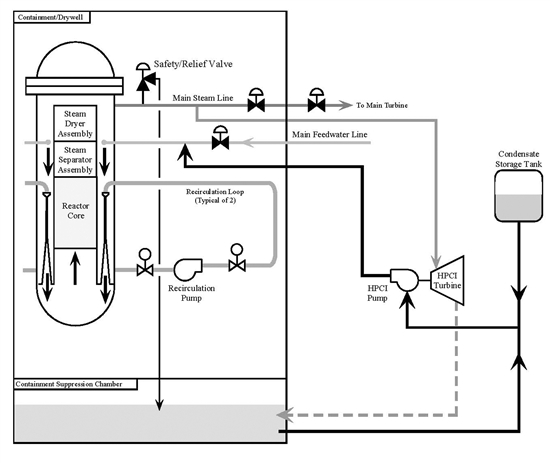
\includegraphics[width=\linewidth]{./graphs/BWR.jpg}
		\column{0.4\textwidth}
		\begin{itemize}
			\small
			\item Start of the transient: closure of the MSIV
			\item Reactor will automatically SCRAM if MSIV closed
			\item Conditions:
			\begin{itemize}
				\item 100 ms SCRAM delay
				\item 300 ms SCRAM delay
				\item 500 ms SCRAM delay
				\item no SCRAM (control logic removed from the simulation)
			\end{itemize}
			In the last case: reactor WILL SCRAM, but not from MSIV closure signal
		\end{itemize}
	\end{columns}
	\end{frame}
\begin{frame}{Start of the transient}
	\begin{figure}
		\centering
		\begin{minipage}{.5\textwidth}
			\centering
			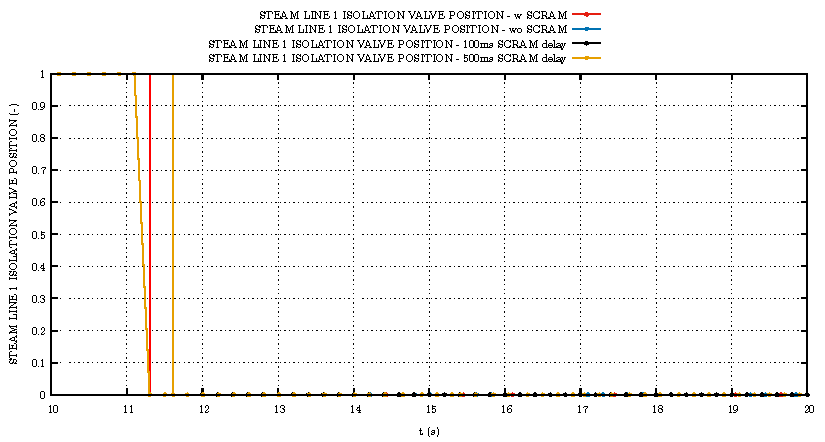
\includegraphics[width=0.7\linewidth]{./graphs/STEAM LINE 1 ISOLATION VALVE POSITION_comp.pdf}
%			\captionof{figure}{A figure}
%			\label{fig:test1}
		\end{minipage}%
		\begin{minipage}{.5\textwidth}
			\centering
			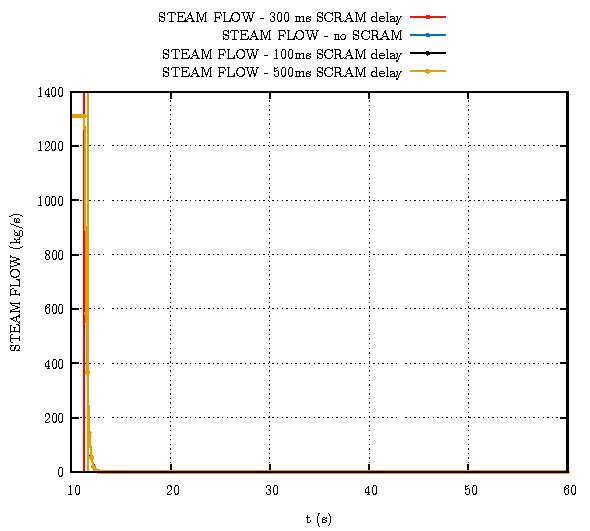
\includegraphics[width=.7\linewidth]{./graphs/STEAM FLOW_comp.pdf}
%			\captionof{figure}{Another figure}
%			\label{fig:test2}
		\end{minipage}
	\end{figure}
	\vspace{-10pt}
	\begin{figure}
	\centering
	\begin{minipage}{.5\textwidth}
		\centering
		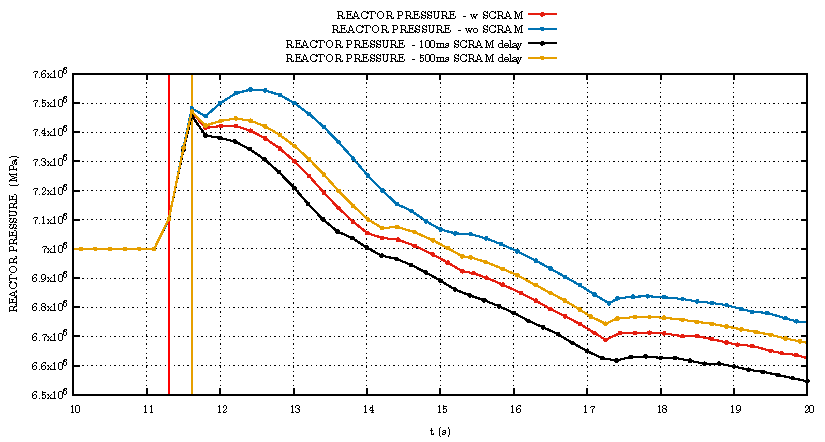
\includegraphics[width=0.7\linewidth]{./graphs/REACTOR PRESSURE _comp.pdf}
		%			\captionof{figure}{A figure}
		%			\label{fig:test1}
	\end{minipage}%
	\begin{minipage}{.5\textwidth}
		\centering
		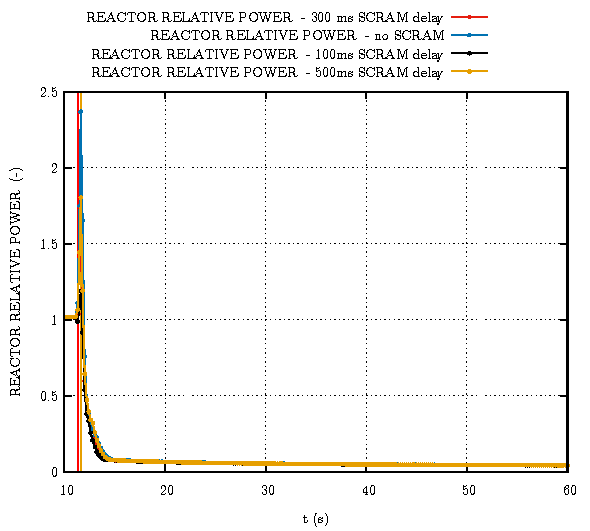
\includegraphics[width=.7\linewidth]{./graphs/REACTOR RELATIVE POWER _comp.pdf}
		%			\captionof{figure}{Another figure}
		%			\label{fig:test2}
	\end{minipage}
\end{figure}
\end{frame}

%\begin{frame}{Pressure relief}
%
%	\begin{figure}
%		\centering
%		\begin{minipage}{.5\textwidth}
%			\centering
%			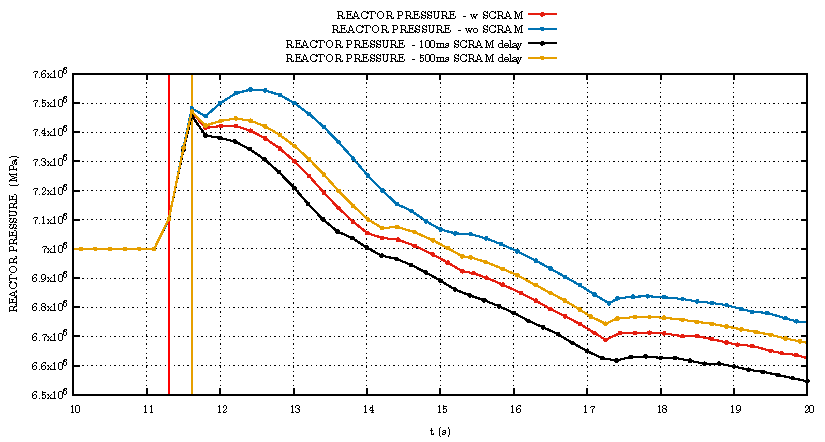
\includegraphics[width=0.7\linewidth]{./graphs/REACTOR PRESSURE _comp.pdf}
%			%			\captionof{figure}{A figure}
%			%			\label{fig:test1}
%		\end{minipage}%
%		\begin{minipage}{.5\textwidth}
%			\centering
%			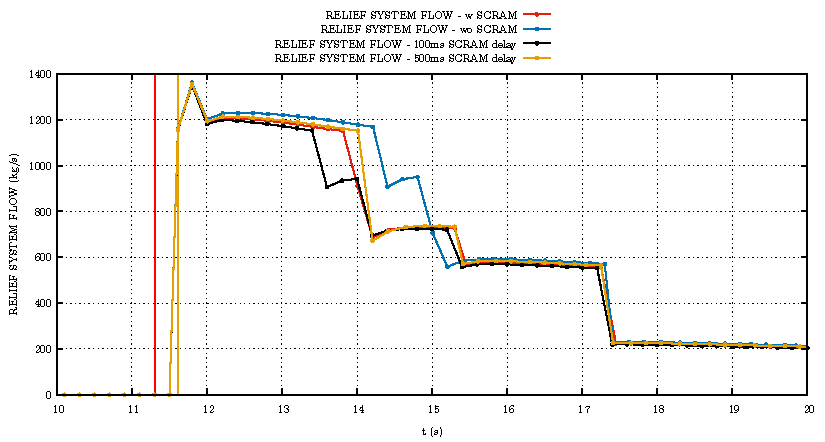
\includegraphics[width=.7\linewidth]{./graphs/RELIEF SYSTEM FLOW_comp.pdf}
%			%			\captionof{figure}{Another figure}
%			%			\label{fig:test2}
%		\end{minipage}
%	\end{figure}
%	\vspace{-10pt}
%	\begin{figure}
%	\centering
%	\begin{minipage}{.5\textwidth}
%		\centering
%		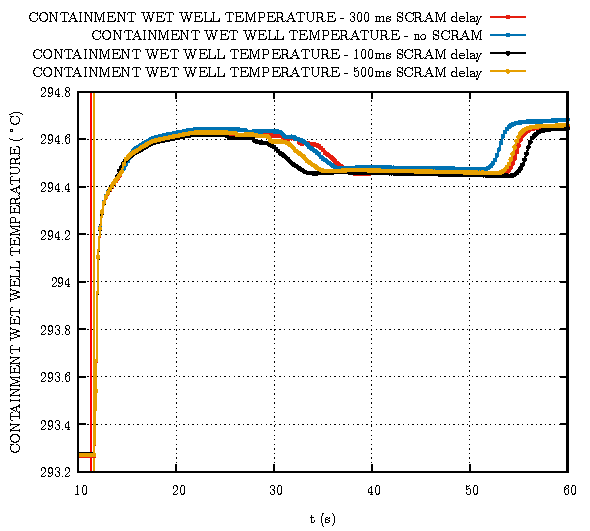
\includegraphics[width=0.7\linewidth]{./graphs/CONTAINMENT WET WELL TEMPERATURE_comp.pdf}
%		%			\captionof{figure}{A figure}
%		%			\label{fig:test1}
%	\end{minipage}%
%	\vspace{-10pt}
%	\begin{minipage}{.5\textwidth}
%		
%		\begin{itemize}
%			\item \small{Closure of relief valves by groups}
%			\item Different rellief procedure for no SCRAM - caused by much higher power rise (nearly 2 times than for 50 ms SCRAM delay)
%		\end{itemize}
%			
%		
%%		\centering
%%		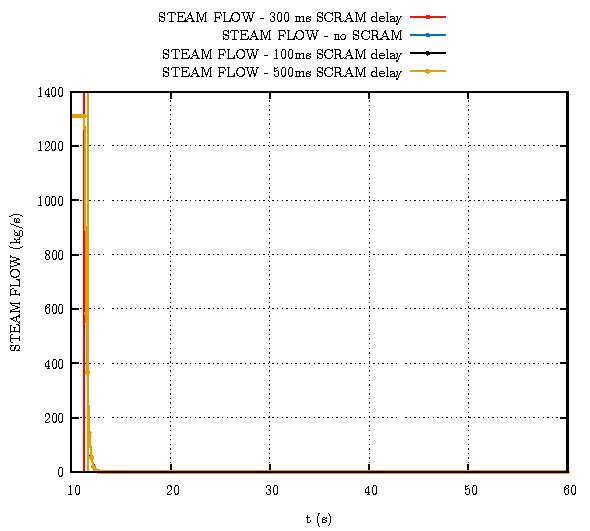
\includegraphics[width=.8\linewidth]{./graphs/STEAM FLOW_comp.pdf}
%		%			\captionof{figure}{Another figure}
%		%			\label{fig:test2}
%	\end{minipage}
%\end{figure}
%\end{frame}


\begin{frame}{Pressure relief}
	
	\begin{figure}
		\centering
		\begin{minipage}{.5\textwidth}
			\centering
			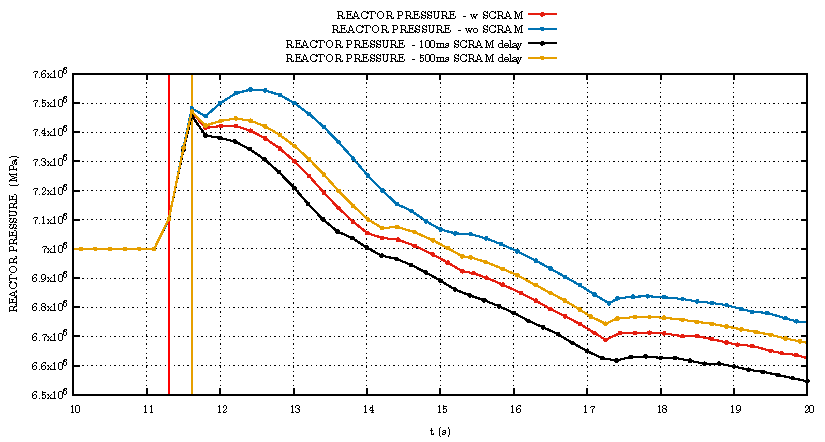
\includegraphics[width=0.7\linewidth]{./graphs/REACTOR PRESSURE _comp.pdf}
			%			\captionof{figure}{A figure}
			%			\label{fig:test1}
		\end{minipage}%
		\begin{minipage}{.5\textwidth}
			\centering
			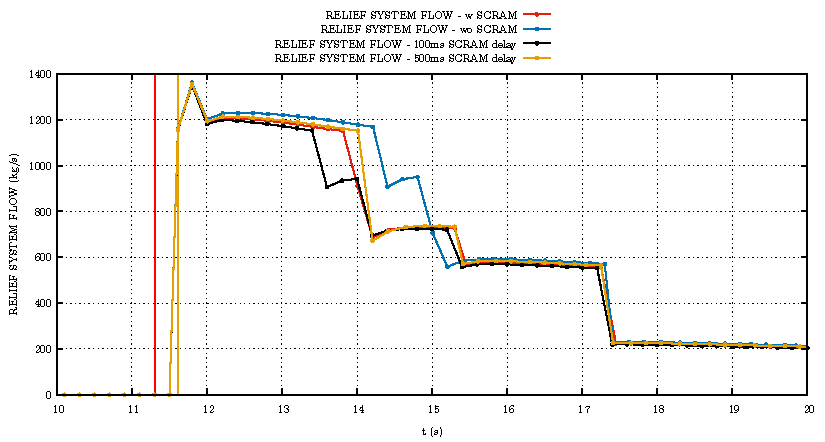
\includegraphics[width=.7\linewidth]{./graphs/RELIEF SYSTEM FLOW_comp.pdf}
			%			\captionof{figure}{Another figure}
			%			\label{fig:test2}
		\end{minipage}
	\end{figure}
	\vspace{-10pt}
	\begin{figure}
		\centering
		\begin{minipage}{.5\textwidth}
			\centering
			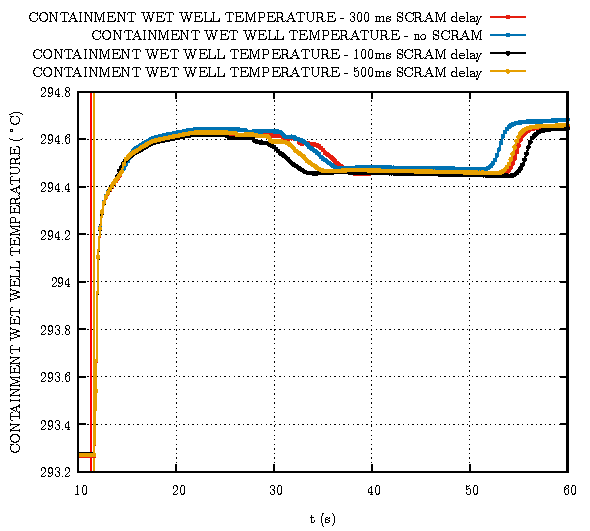
\includegraphics[width=0.7\linewidth]{./graphs/CONTAINMENT WET WELL TEMPERATURE_comp.pdf}
			%			\captionof{figure}{A figure}
			%			\label{fig:test1}
		\end{minipage}%
		\begin{minipage}{.5\textwidth}
			\begin{itemize}
				\small{
				\item Closure of relief valves by groups
				\item Different rellief procedure for no SCRAM - caused by much higher power rise (nearly 2 times than for 50 ms SCRAM delay)}
			\end{itemize}
			%		\centering
			%		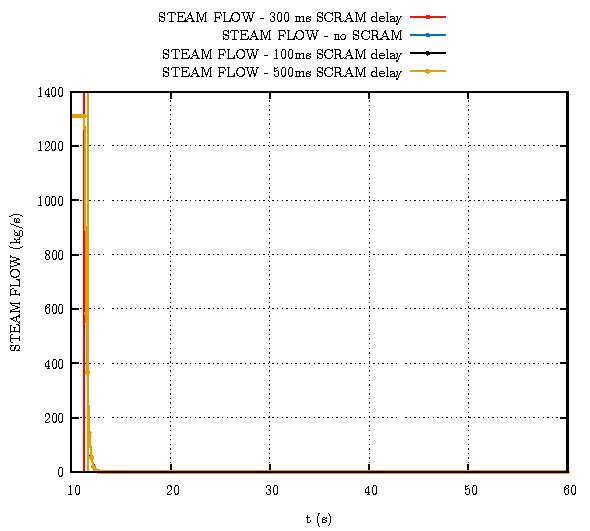
\includegraphics[width=.8\linewidth]{./graphs/STEAM FLOW_comp.pdf}
			%			\captionof{figure}{Another figure}
			%			\label{fig:test2}
		\end{minipage}
	\end{figure}
\end{frame}

\begin{frame}{What happens in the reactor?}
	
	\begin{figure}
		\centering
		\begin{minipage}{.5\textwidth}
			\centering
			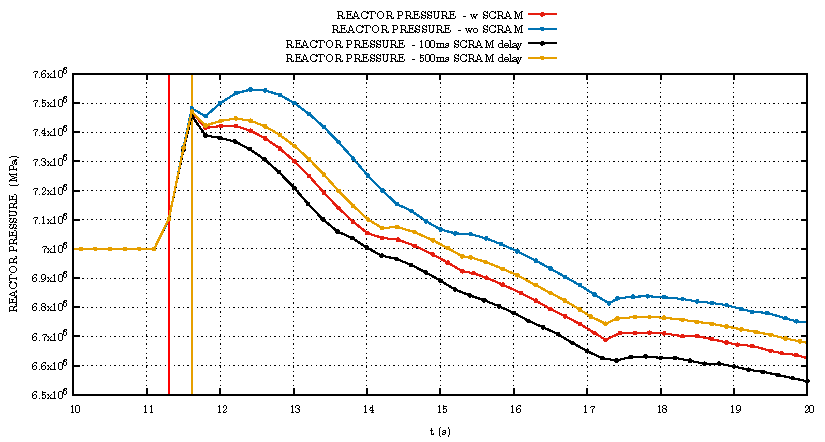
\includegraphics[width=0.7\linewidth]{./graphs/REACTOR PRESSURE _comp.pdf}
			%			\captionof{figure}{A figure}
			%			\label{fig:test1}
		\end{minipage}%
		\begin{minipage}{.5\textwidth}
			\centering
			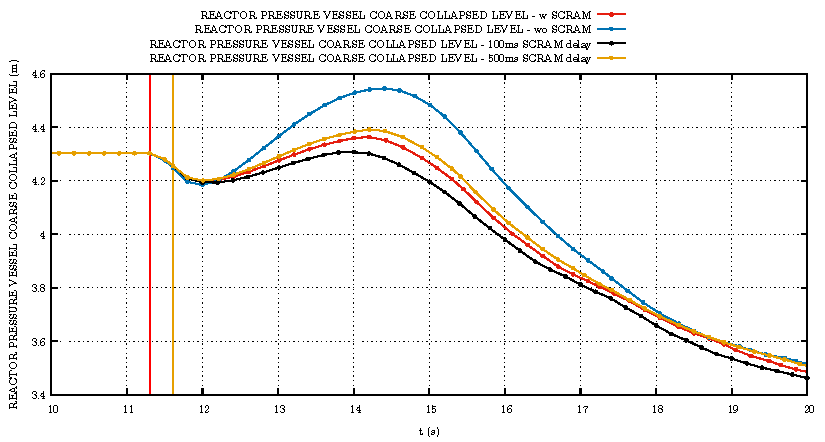
\includegraphics[width=.7\linewidth]{./graphs/REACTOR PRESSURE VESSEL COARSE COLLAPSED LEVEL_comp.pdf}
			%			\captionof{figure}{Another figure}
			%			\label{fig:test2}
		\end{minipage}
	\end{figure}
	\vspace{-10pt}
	\begin{figure}
		\centering
		\begin{minipage}{.5\textwidth}
			\centering
			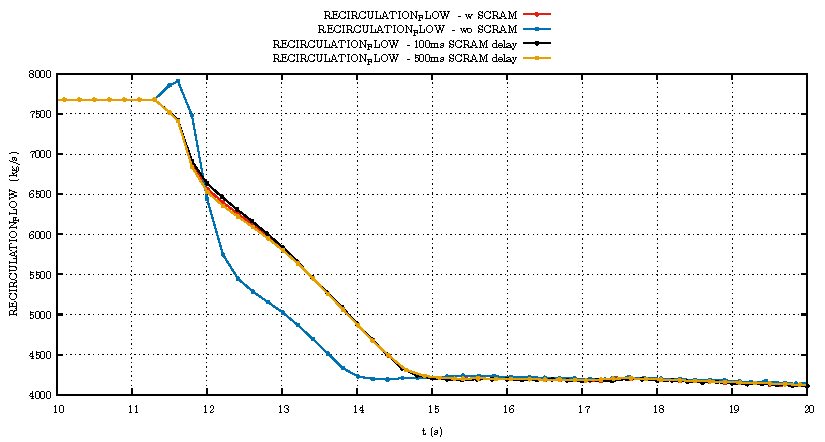
\includegraphics[width=0.7\linewidth]{./graphs/RECIRCULATION_FLOW _comp.pdf}
			%			\captionof{figure}{A figure}
			%			\label{fig:test1}
		\end{minipage}%
		\begin{minipage}{.5\textwidth}
			
			
					\centering
					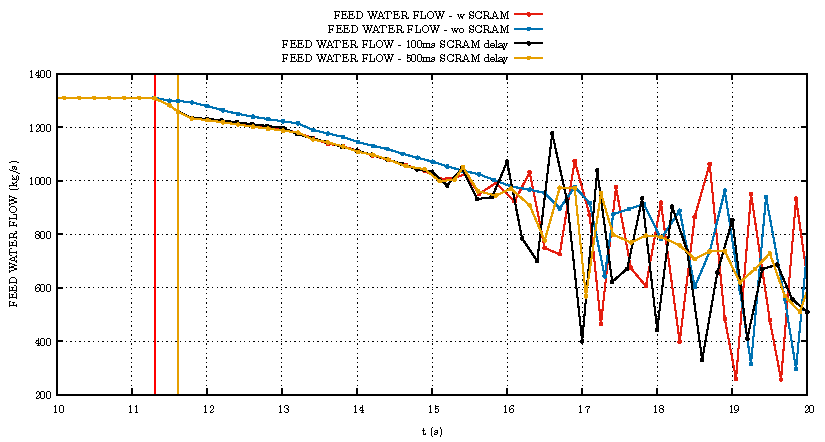
\includegraphics[width=.7\linewidth]{./graphs/FEED WATER FLOW_comp.pdf}
%						\captionof{figure}{Another figure}
%						\label{fig:test2}
		\end{minipage}
	\end{figure}
\end{frame}

\begin{frame}{What causes the oscillations in the feed water flow?}
	
	\begin{figure}
		\centering
		\begin{minipage}{.5\textwidth}
			\centering
			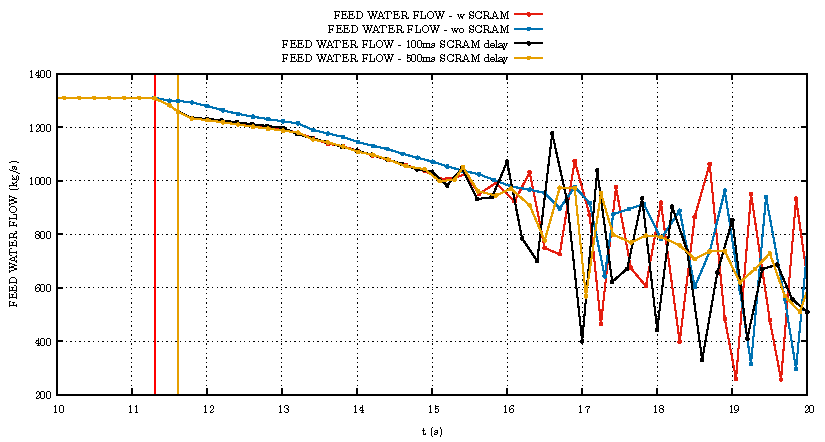
\includegraphics[width=0.7\linewidth]{./graphs/FEED WATER FLOW_comp.pdf}
			%			\captionof{figure}{A figure}
			%			\label{fig:test1}
		\end{minipage}%
		\begin{minipage}{.5\textwidth}
			\centering
			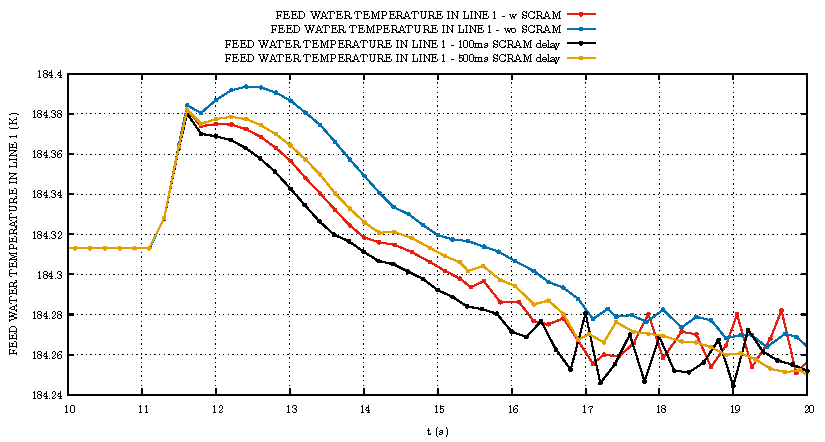
\includegraphics[width=.7\linewidth]{./graphs/FEED WATER TEMPERATURE IN LINE 1_comp.pdf}
			%			\captionof{figure}{Another figure}
			%			\label{fig:test2}
		\end{minipage}
	\end{figure}
	\vspace{-10pt}
	\begin{figure}
		\centering
		\begin{minipage}{.5\textwidth}
			\centering
			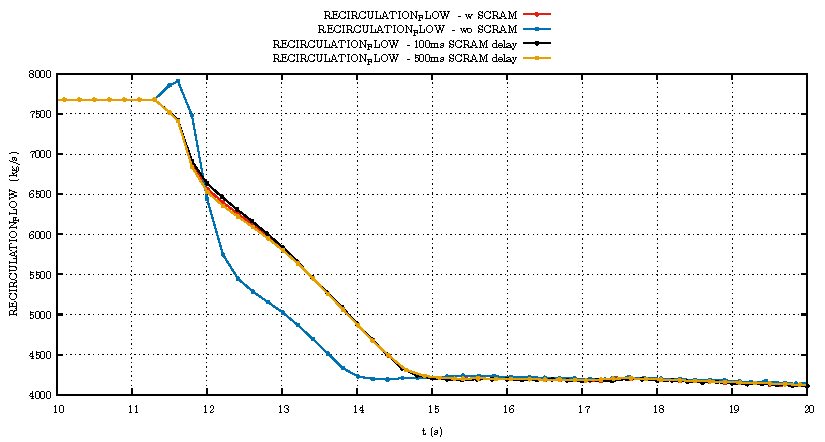
\includegraphics[width=0.7\linewidth]{./graphs/RECIRCULATION_FLOW _comp.pdf}
			%			\captionof{figure}{A figure}
			%			\label{fig:test1}
		\end{minipage}%
		\begin{minipage}{.5\textwidth}
			
			
			\centering
			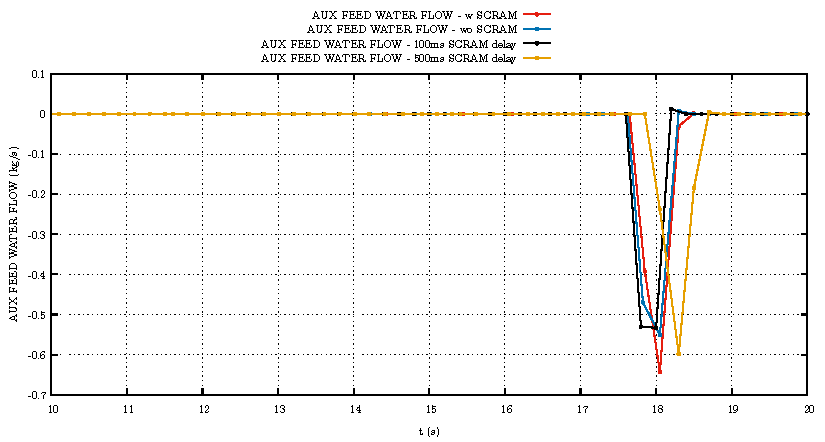
\includegraphics[width=.7\linewidth]{./graphs/AUX FEED WATER FLOW_comp.pdf}
			%						\captionof{figure}{Another figure}
			%						\label{fig:test2}
		\end{minipage}
	\end{figure}
\end{frame}
%\begin{frame}{Steam line break valve 1 mass flow}
%	\begin{figure}
%		\centering
%		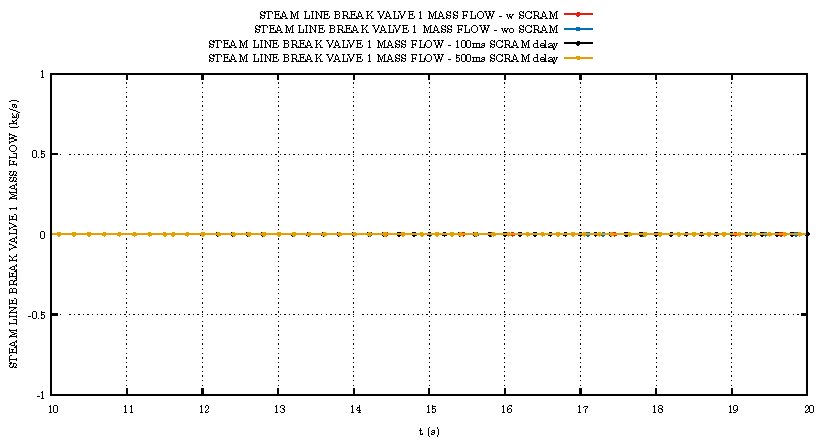
\includegraphics[width=\textwidth]{./graphs/STEAM LINE BREAK VALVE 1 MASS FLOW_comp.pdf}
%		
%	\end{figure}
%\end{frame}
%
%\begin{frame}{Steam line break valve 2 mass flow}
%	\begin{figure}
%		\centering
%		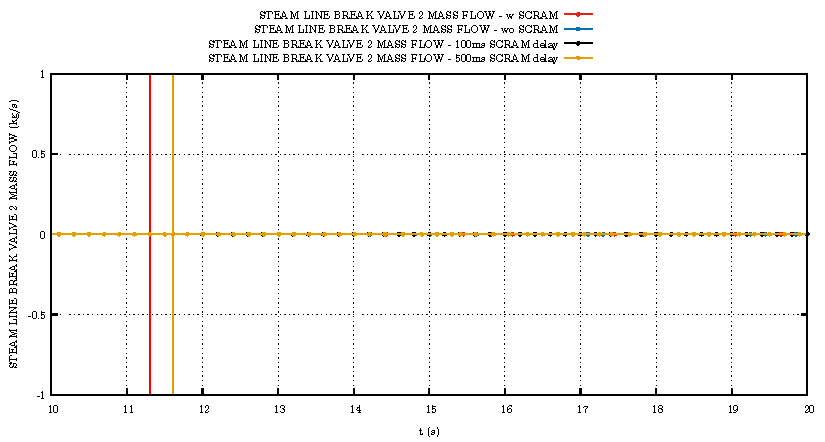
\includegraphics[width=\textwidth]{./graphs/STEAM LINE BREAK VALVE 2 MASS FLOW_comp.pdf}
%		
%	\end{figure}
%\end{frame}





%
\begin{frame}{The natural convection instability?}
	\begin{figure}
	\centering
	\begin{minipage}{.5\textwidth}
		\centering
		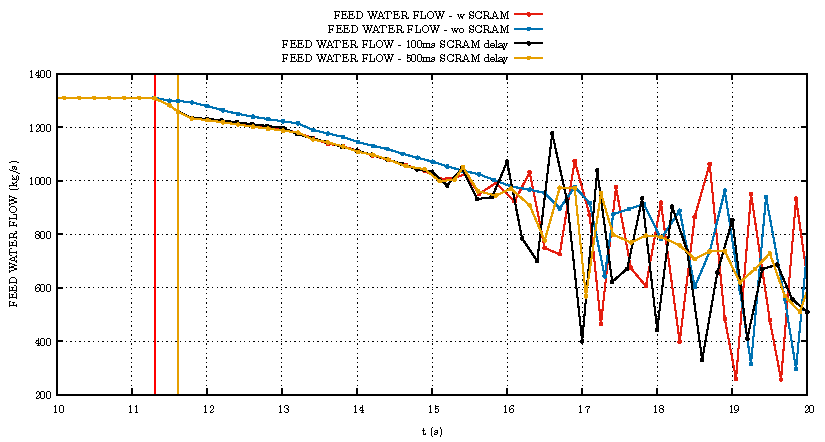
\includegraphics[width=0.7\linewidth]{./graphs/FEED WATER FLOW_comp.pdf}
		%			\captionof{figure}{A figure}
		%			\label{fig:test1}
	\end{minipage}%
	\begin{minipage}{.5\textwidth}
		\centering
		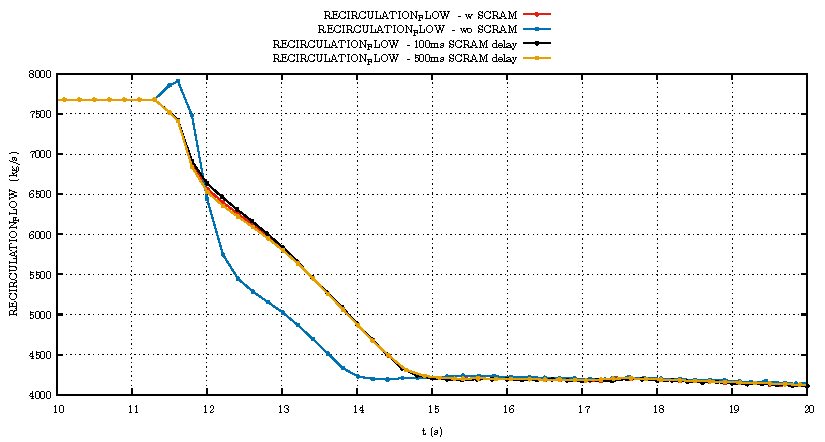
\includegraphics[width=.7\linewidth]{./graphs/RECIRCULATION_FLOW _comp.pdf}
		%			\captionof{figure}{Another figure}
		%			\label{fig:test2}
	\end{minipage}
\end{figure}
\vspace{-10pt}
%\begin{figure}
%	\centering
%	\begin{minipage}{.5\textwidth}
%		\centering
%		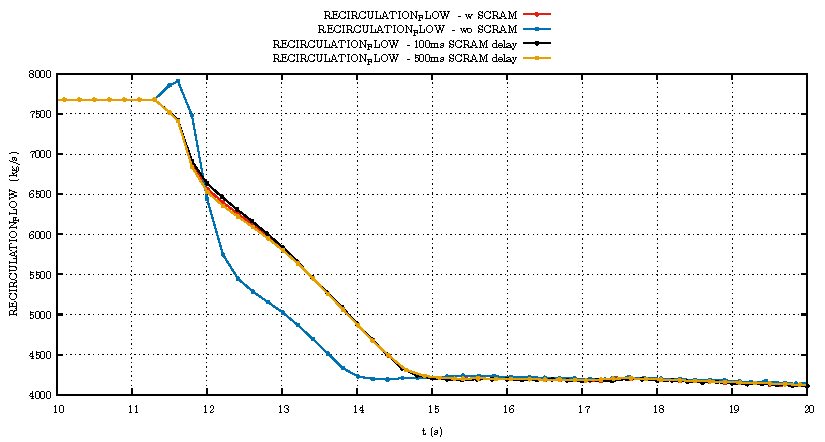
\includegraphics[width=0.7\linewidth]{./graphs/RECIRCULATION_FLOW _comp.pdf}
%		%			\captionof{figure}{A figure}
%		%			\label{fig:test1}
%	\end{minipage}%
%	\begin{minipage}{.5\textwidth}
%		
%		
%		\centering
%		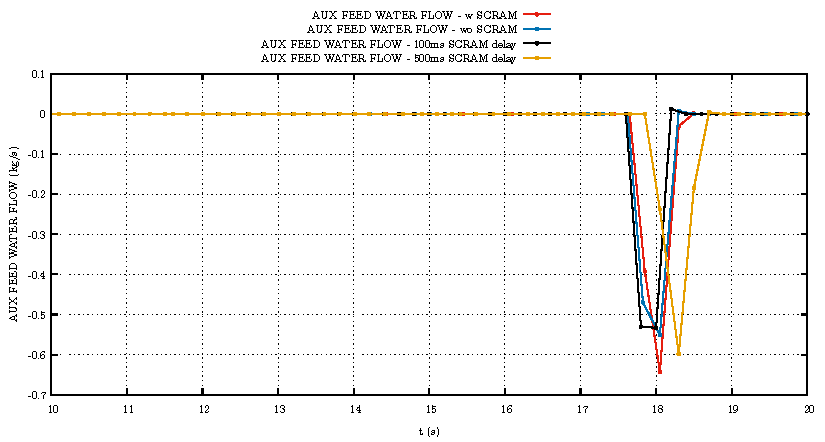
\includegraphics[width=.7\linewidth]{./graphs/AUX FEED WATER FLOW_comp.pdf}
%		%						\captionof{figure}{Another figure}
%		%						\label{fig:test2}
%	\end{minipage}
%\end{figure}
	
\end{frame}




\begin{frame}{Temperatures}
		\begin{figure}
		\centering
		\begin{minipage}{.5\textwidth}
			\centering
			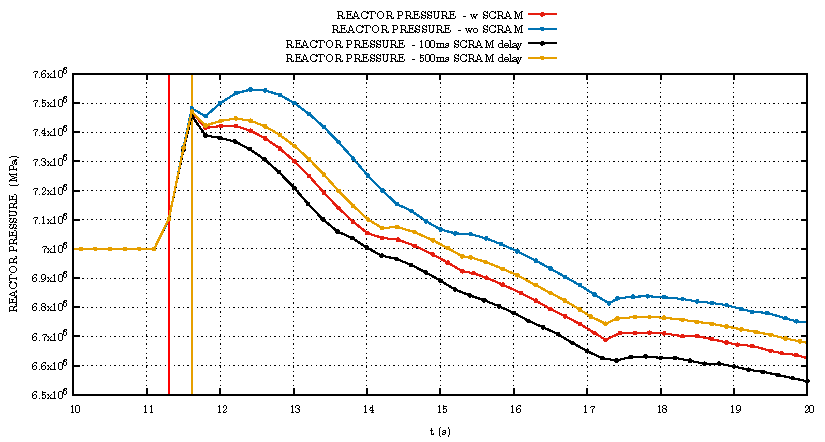
\includegraphics[width=0.7\linewidth]{./graphs/REACTOR PRESSURE _comp.pdf}
			%			\captionof{figure}{A figure}
			%			\label{fig:test1}
		\end{minipage}%
		\begin{minipage}{.5\textwidth}
			\centering
			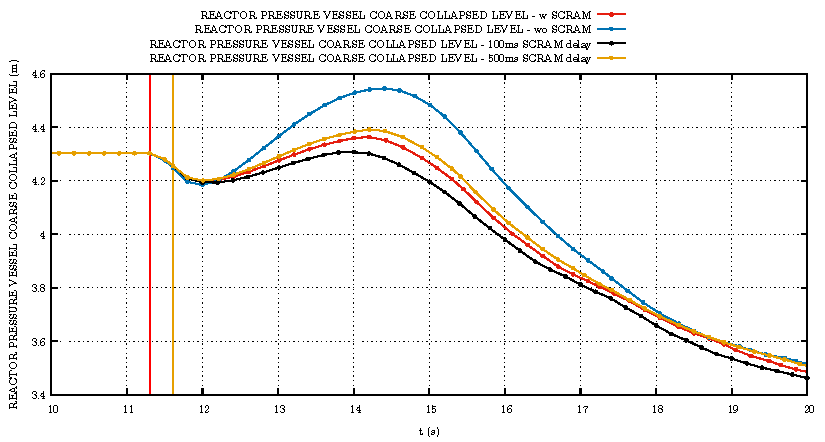
\includegraphics[width=.7\linewidth]{./graphs/REACTOR PRESSURE VESSEL COARSE COLLAPSED LEVEL_comp.pdf}
			%			\captionof{figure}{Another figure}
			%			\label{fig:test2}
		\end{minipage}
	\end{figure}
	\vspace{-10pt}
	\begin{figure}
		\centering
		\begin{minipage}{.5\textwidth}
			\centering
			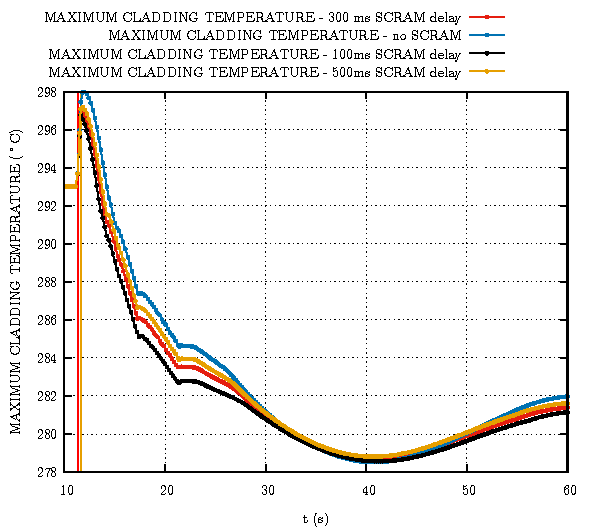
\includegraphics[width=0.7\linewidth]{./graphs/MAXIMUM CLADDING TEMPERATURE_comp.pdf}
			%			\captionof{figure}{A figure}
			%			\label{fig:test1}
		\end{minipage}%
		\begin{minipage}{.5\textwidth}
			
			
			\centering
			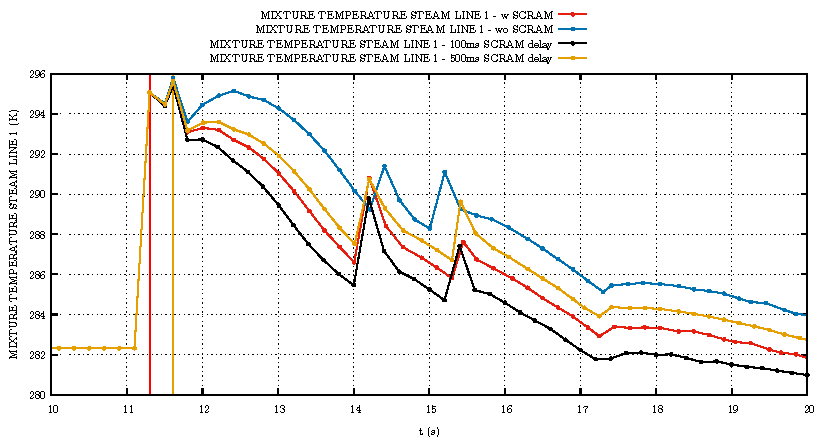
\includegraphics[width=.7\linewidth]{./graphs/MIXTURE TEMPERATURE STEAM LINE 1_comp.pdf}
			%						\captionof{figure}{Another figure}
			%						\label{fig:test2}
		\end{minipage}
	\end{figure}
\end{frame}

%\begin{frame}{RPV coarse level measurement}
%	\begin{figure}
%		\centering
%		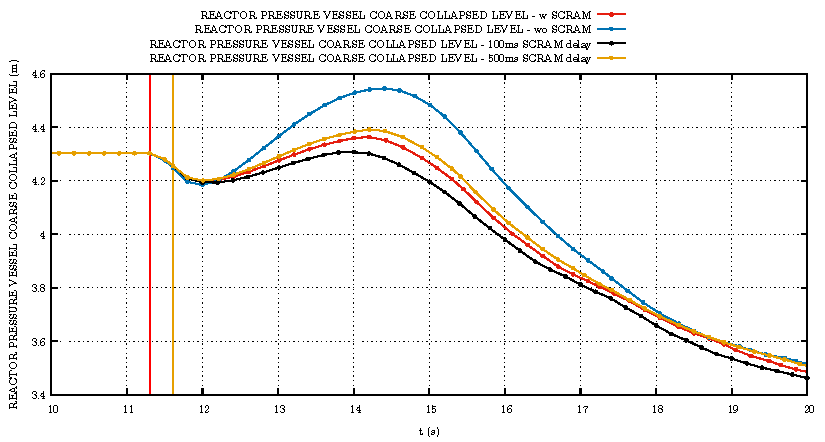
\includegraphics[width=\textwidth]{./graphs/REACTOR PRESSURE VESSEL COARSE COLLAPSED LEVEL_comp.pdf}
%		
%	\end{figure}
%	
%\end{frame}
%
%
%\begin{frame}{Dry well temperature}
%	\begin{figure}
%		\centering
%		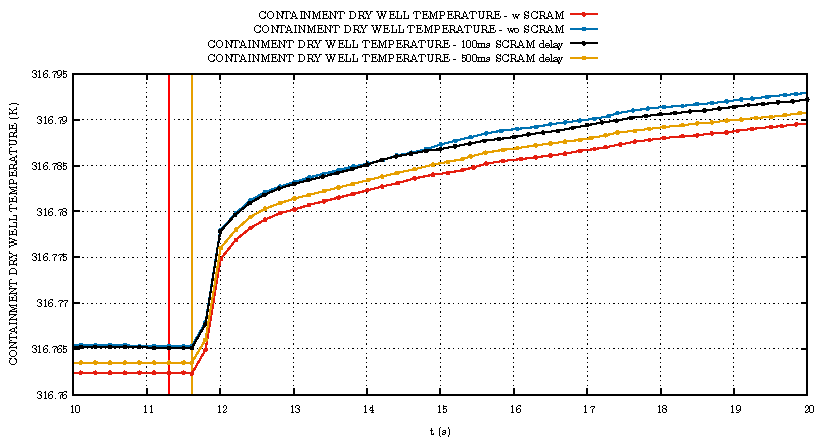
\includegraphics[width=\textwidth]{./graphs/CONTAINMENT DRY WELL TEMPERATURE_comp.pdf}
%		
%	\end{figure}
%	
%\end{frame}
%\begin{frame}{Wet well temperature}
%	\begin{figure}
%		\centering
%		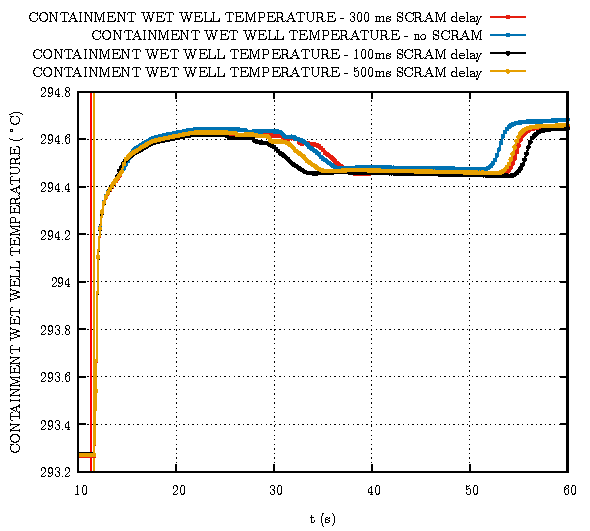
\includegraphics[width=\textwidth]{./graphs/CONTAINMENT WET WELL TEMPERATURE_comp.pdf}
%		
%	\end{figure}
%	
%\end{frame}
%
%
%
%\begin{frame}{Auxiliary feed water flow}
%	\begin{figure}
%		\centering
%		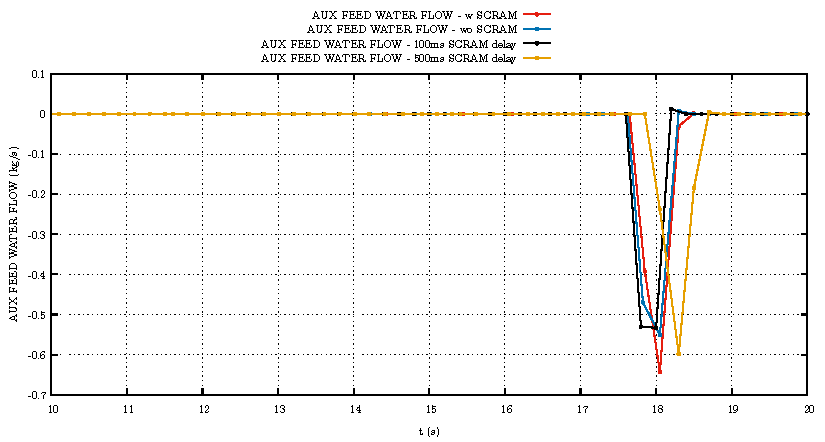
\includegraphics[width=\textwidth]{./graphs/AUX FEED WATER FLOW_comp.pdf}
%		
%	\end{figure}
%	
%\end{frame}
%
%
%\begin{frame}{Feed water temperature 1}
%	\begin{figure}
%		\centering
%		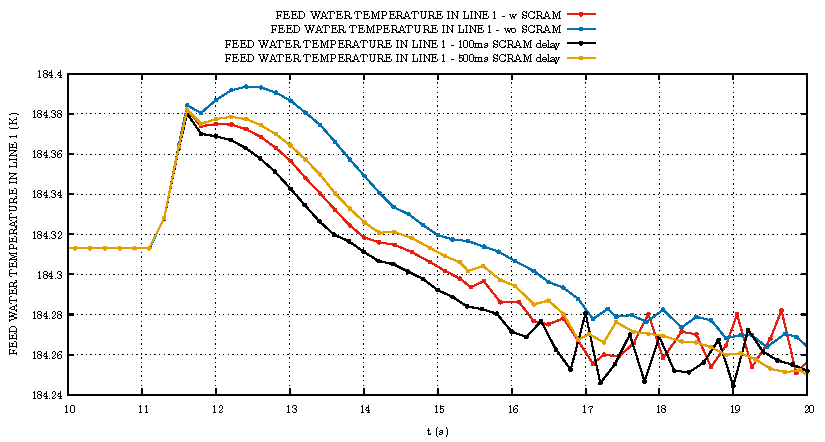
\includegraphics[width=\textwidth]{./graphs/FEED WATER TEMPERATURE IN LINE 1_comp.pdf}
%		
%	\end{figure}
%	
%\end{frame}
%
%
%
%
%
%
%
%
%\begin{frame}{Steam flow}
%	\begin{figure}
%		\centering
%		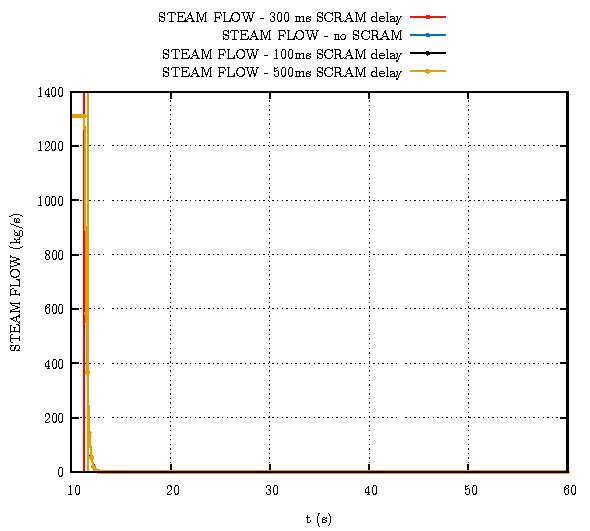
\includegraphics[width=\textwidth]{./graphs/STEAM FLOW_comp.pdf}
%		
%	\end{figure}
%	
%\end{frame}
%
%
%
%
%\begin{frame}{MSIV position}
%	\begin{figure}
%		\centering
%		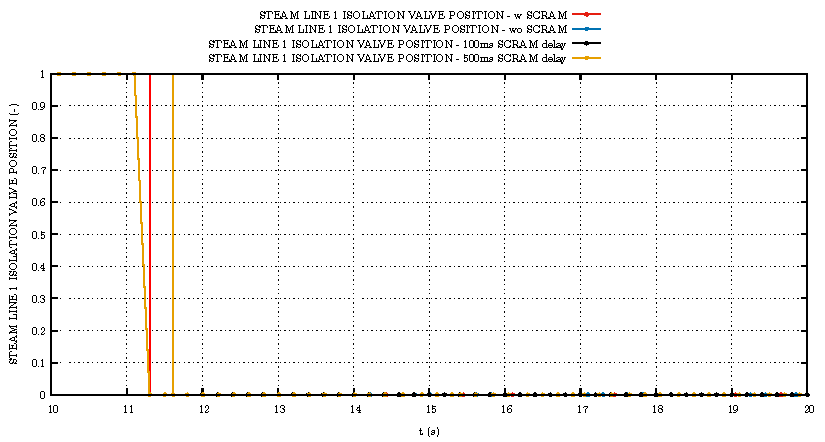
\includegraphics[width=\textwidth]{./graphs/STEAM LINE 1 ISOLATION VALVE POSITION_comp.pdf}
%		
%	\end{figure}
%	
%\end{frame}
%
%
%
%
%
%
%
%
%\begin{frame}{Maximum cladding temperature}
%	\begin{figure}
%			\centering
%			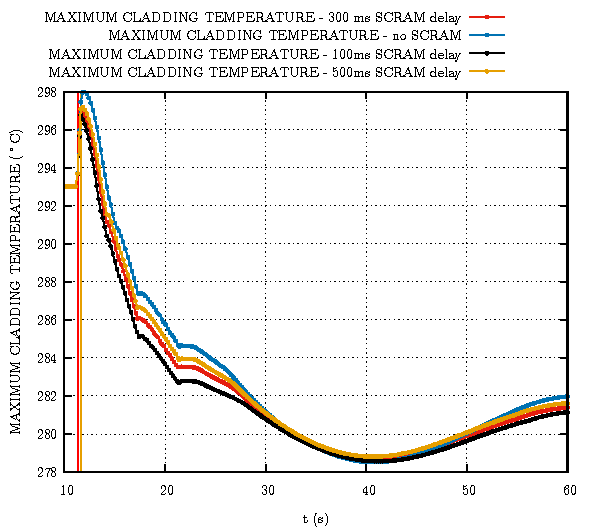
\includegraphics[width=\textwidth]{./graphs/MAXIMUM CLADDING TEMPERATURE_comp.pdf}
%			
%		\end{figure}
%	
%\end{frame}






%\begin{frame}{Steam mixture temperature}
%	\begin{figure}
%		\centering
%		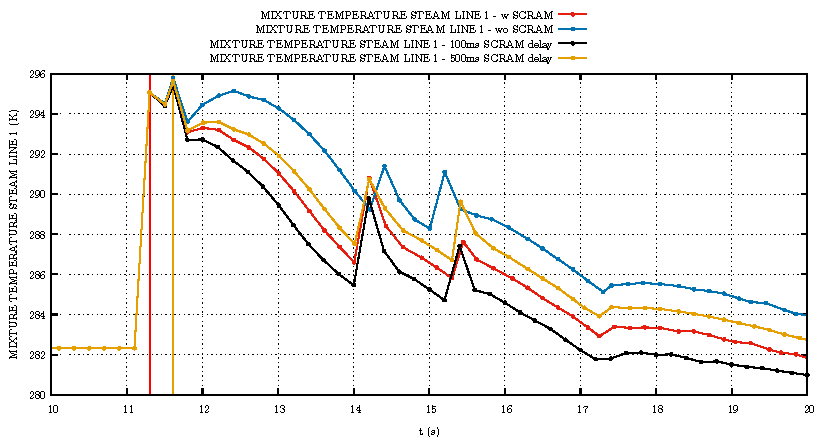
\includegraphics[width=\textwidth]{./graphs/MIXTURE TEMPERATURE STEAM LINE 1_comp.pdf}
%		
%	\end{figure}
%	
%\end{frame}


%\begin{frame}{Feed water temperature}
%	\begin{figure}
%		\centering
%		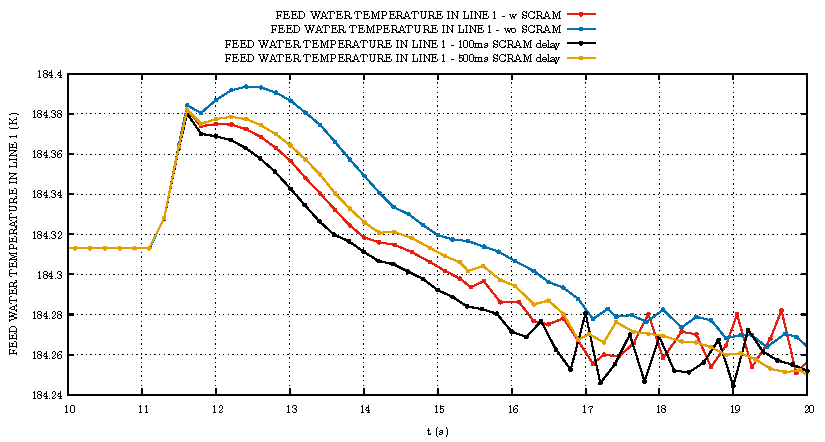
\includegraphics[width=\textwidth]{./graphs/FEED WATER TEMPERATURE IN LINE 1_comp.pdf}
%		
%	\end{figure}
%	
%\end{frame}
%\begin{frame}{Feed water temperature}
%	\begin{figure}
%		\centering
%		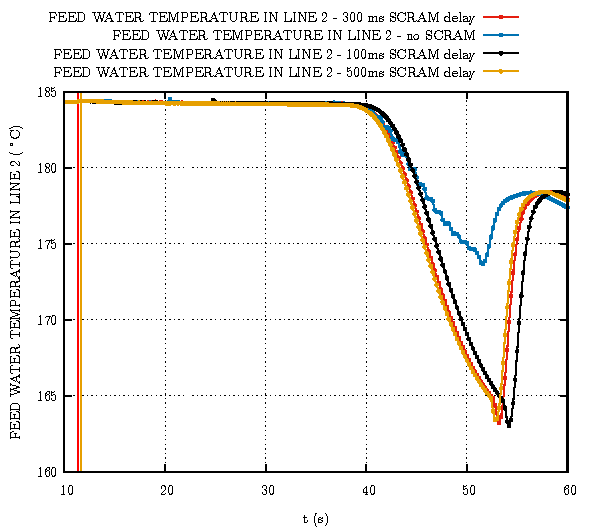
\includegraphics[width=\textwidth]{./graphs/FEED WATER TEMPERATURE IN LINE 2_comp.pdf}
%		
%	\end{figure}
%	
%\end{frame}
%






\begin{frame}
\Large{{Thanks for attention!}}
\vspace{0.5cm}
\hrule
\vspace{3cm}
\end{frame}

\nologo


\end{document}
